\section{Measurement Scope and Implications}
\label{sec:scope}

\subsection{Resilience and Infrastructure Implications}
\label{subsec:resilience-implications}

Routing diversity and corridor breadth capture distinct structures: 81
service-facing units project broad network alternatives onto narrow feasible
coastal directions, whereas 158 retain distributed support at both layers.
Exposure links service localization and interconnection to the frequency of
inter-region access; concentration links landing-region diversification to the
breadth of physical support. Together they locate country-service populations
relevant to replica placement, peering, and international connectivity planning.

The paired view also distinguishes two intervention points. Deploying a closer
service instance or changing interconnection can reduce exposure by keeping
more paths within a region. Adding access through distinct landing regions can
broaden the corridor distribution of paths that continue to cross regions.

\subsection{Physical Mapping Resolution}
\label{subsec:mapping-resolution-scope}

Each segment records one mapping-resolution state. At 30~km, 57.9\% of
candidate-bearing segments have one corridor and 42.1\% divide unit mass across
a bounded set. Segments with no feasible corridor or incomplete construction
inputs remain separate in pipeline accounting. Corridor, exact landing-pair,
and cable identities remain linked in the outputs, supporting analysis across
physical resolutions.

Uniform allocation gives each observed segment one total unit of influence.
Repeated support for the same corridor accumulates across traces, while
segments with several feasible corridors distribute their unit across that
finite set. Aggregate concentration thus combines observation frequency with
candidate overlap.

\subsection{Landing-Region Resolution Sensitivity}
\label{subsec:resolution-sensitivity}

To assess resolution sensitivity, we vary maximum landing-region diameter over
10, 20, 30, 40, and 50~km while holding the 50-km endpoint catchment and 5-ms
RTT tolerance fixed. Exact landing-pair and cable candidate sets are identical
on baseline-shared segments (mean Jaccard 1.0), isolating corridor grouping
resolution.

The single-corridor share is 46.2\%, 47.4\%, and 54.8\% at 10-30~km, rising to
90.1\% and 94.8\% at 40-50~km. Shared-cohort Top-2 share follows the same
transition: 53.6\%, 62.8\%, and 64.4\%, then 81.6\% and 84.9\%. From 30 to
40~km, these measures increase by 35.3 and 17.2 percentage points as spatial
aggregation merges candidate support into fewer corridors. The 10-30-km
settings preserve a fine-grained coastal view; the 40-50-km settings form
larger regions and concentrate the same landing-pair support.

\begin{figure}[t]
  \centering
  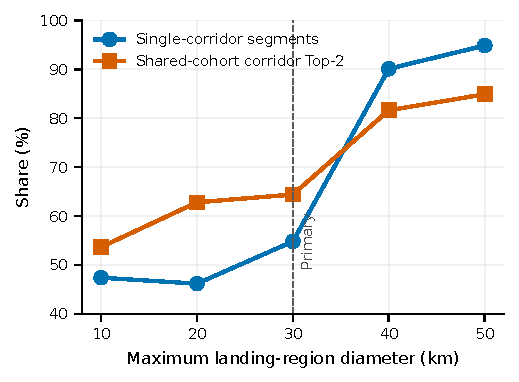
\includegraphics[width=0.84\columnwidth]{figures/fig_sensitivity_diameter.pdf}
  \caption{Landing-region diameter sensitivity.}
  \label{fig:diameter-sensitivity}
\end{figure}

\subsection{Measurement Scope}
\label{subsec:measurement-scope}

RIPE Atlas probe density varies across countries and networks; reported
quantities are observation-weighted over participating probes in the aligned
window. DNS Roots and applications form service-specific populations, while
MSM 5051 and 5151 retain dynamic multi-target populations as topology
references. Anycast observations integrate deployed footprint, BGP selection,
interconnection, and source-network context.

The primary corridor distribution includes domestic and international inter-
region candidates, with the corresponding label retained per segment. All
measurements cover 00:00-01:00 UTC on July~1, 2026 and align with IP, AS,
cable-lifecycle, and deployment metadata. Corridor concentration quantifies
geographic candidate support; cable multiplicity, landing-station redundancy,
hazard correlation, rerouting capacity, and repair processes supply additional
operational dimensions.

The snapshot provides a common temporal basis across all service families.
Repeating the aligned construction over time can track changes caused by
routing, service deployment, or cable lifecycle events at the same country-
measurement granularity.

\subsection{Ethics and Reproducibility}
\label{subsec:ethics-reproducibility}

The study uses archived public RIPE Atlas measurements and infrastructure
metadata and reports aggregate country-measurement statistics. Released
measurement IDs, configuration values, resolution states, pipeline counts, and
scripts reconstruct the primary tables and figures from versioned inputs.
